\documentclass[a4paper,12pt]{article}
\usepackage{graphicx}
\usepackage{listings}
\usepackage{xcolor}
\usepackage{amsmath}
\usepackage{booktabs}
\usepackage{hyperref}
\usepackage{geometry} % Adjust page margins
\geometry{margin=1in} % Set 1-inch margins
\usepackage{xcolor}
\usepackage{listings}

\definecolor{codegreen}{rgb}{0,0.6,0}
\definecolor{codegray}{rgb}{0.5,0.5,0.5}
\definecolor{codepurple}{rgb}{0.58,0,0.82}
\definecolor{backcolour}{rgb}{0.95,0.95,0.92}

\lstdefinestyle{mystyle}{
    backgroundcolor=\color{backcolour},   
    commentstyle=\color{codegreen},
    keywordstyle=\color{magenta},
    numberstyle=\tiny\color{codegray},
    stringstyle=\color{codepurple},
    basicstyle=\ttfamily\footnotesize,
    breakatwhitespace=false,         
    breaklines=true,                 
    captionpos=b,                    
    keepspaces=true,                 
    numbers=left,                    
    numbersep=5pt,                  
    showspaces=false,                
    showstringspaces=false,
    showtabs=false,                  
    tabsize=2
}

\lstset{style=mystyle}

\title{Surface Brightness Profile Extraction for A2163 \\ Using CIAO and Python}
\author{Prepared by Anurag Garg}
\date{\today}

\begin{document}
\maketitle

\section{Introduction}
This report documents the step-by-step procedure for processing Chandra X-ray data for A2163, extracting the surface brightness profile, and fitting a $\beta$-model using Python. The analysis was performed using CIAO 4.17.

\section{CIAO Commands and Usage}

\subsection{Loading CIAO Environment}
To ensure CIAO is correctly set up:
\begin{lstlisting}[language=bash]
source $CIAO_DIR$/bin/ciao.sh
\end{lstlisting}
This initializes CIAO and sets the correct calibration database (CALDB).

\subsection{Downloading Data Product}
We are using Abell 2163, cluster of galaxy, and will be calculating its surface brightness. To download its data product using \textbf{Chandra archive retrival tool} Figure - \label{fig:Chanda Archive reterival tool}, we need to visit \url{https://cda.harvard.edu/chaser/}.

For Abell 2163 we found two different observations recorded under Table - \ref{table: Data Product details}
\begin{enumerate}
    \item \textbf{OBSID:} 545
    \item \textbf{OBSID:} 1653
\end{enumerate}

Using the details or following commands we estimated the date and exposure for both the products

\begin{lstlisting}[language=bash]
    dmkeypar acisf00545N005_evt2.fits EXPOSURE echo+
    >>> 9445.9239062939
    dmkeypar acisfXXXXX_evt2.fits DATE-OBS echo+
    >>> 2000-07-29T11:11:02

    dmkeypar acisf01653N004_evt2.fits EXPOSURE echo+
    >>> 71147.089259333
    dmkeypar acisf01653N004_evt2.fits DATE-OBS echo+
    >>> 2001-06-16T11:39:11
\end{lstlisting}

Since the data product with the OBSID 1653 is latest and with larger exposure, we decided to use it.

\subsection{Reprocessing Chandra Data}
The \textbf{chandra\_repro} reprocessing script automates the recommended data processing steps presented in the CIAO analysis threads. The script reads data from the standard data distribution (e.g. primary and secondary directories) and creates a new bad pixel file, a new level=2 event file, and a new level=2 Type II PHA file with the appropriate response files (grating data only).

\textbf{chandra\_repro} may be used to reprocess any ACIS and HRC imaging or grating data.

There are parameters to control certain reprocessing steps, such as creating the new bad pixel file or destreaking the data. Users who wish to have finer-grained control over the reprocessing parameters should instead follow the step-by-step instructions in the CIAO Data Preparation Threads.

\begin{lstlisting}[language=bash]
chandra_repro indir=data/1653 outdir=data/1653/repro cleanup=no mode=h verbose=1
\end{lstlisting}

Check the reprocessed data
\begin{lstlisting}[language=bash]
    dmlist acisf01653_repro_evt2.fits header | grep 'chandra_repro'
\end{lstlisting}


\subsection{Generating an Exposure Map}
The fluximage script creates exposure-corrected images of an ACIS or HRC observation given an events file and one or more energy bands. It automates the creation of the aspect histogram, instrument, and exposure maps. The output image size can be automatically chosen to cover all the data in the observation, or it can be set to match an existing image. For HRC-I observations, the HRC background files from the Chandra CALDB are used - if installed - to subtract off the particle background and so reduce the ring artifacts that can be seen in HRC-I data (this can be turned off by setting the hidden background parameter to "none").

For recently-processed data the script can be run with only two parameters: for example
\begin{lstlisting}[language=bash]
cd data/1653
fluximage repro/acisf01653_repro_evt2.fits outroot=fluxed/ binsize=4 clobber=yes
\end{lstlisting}

The fluximage tool in CIAO processes the raw event files (evt2.fits) to generate exposure-corrected images, which allow for accurate comparison of flux across the field of view. The raw event data contains photon counts, but without corrections for instrumental effects, these counts do not directly represent the true flux.

\subsection{Finding the X-ray Centroid}
To get a centroid, we need to follow section 7.9 from the given file:

\begin{lstlisting}[language=bash]
    gs Documents/ciao_help_files/Chandra Analysis stepwise.pdf    
\end{lstlisting}

The centroid for source Abell 2163 is at \textbf{4253.6, 4461.9}.

After getting the peak and centroid, we need to follow the tutorial given in the following file:

\begin{lstlisting}[language=bash]
    gs Documents/ciao_help_files/Obtain and Fit a Radial Profile - CIAO 4.17.pdf
\end{lstlisting}

The above command gives the physical coordinates of the pixel with max value. Comparison between Current X-ray Centroid and Brightest X-ray Pixel is recording in Table - \ref{tab:Centroid comparision for A2163}

\subsection{Extracting Surface Brightness Profile}
To extract the surface brightness profile or the radial profile, we need to use \textbf{dmextract}. We need the following files:
\begin{enumerate}
    \item event = 2 file (acisf01653\_repro\_evt2.fits)
    \item region file (annuli.reg)
    \item background file. Will be using \textbf{blanksky}
\end{enumerate}

\begin{lstlisting}[language=bash]
    blanksky evtfile="acisf01653_repro_evt2.fits" outfile=1653_blank.evt tmpdir=./ mode=h
\end{lstlisting}

It is now possible to run dmextract to extract the radial profiles:

\begin{lstlisting}[language=bash]
punlearn dmextract
pset dmextract infile="acis_1653_evt2.fits[bin sky=@annuli.reg]"
pset dmextract outfile=1653_rprofile.fits
pset dmextract bkg=""
pset dmextract opt=generic
dmextract
Input event file  (acis_1653_evt2.fits[bin sky=@annuli.reg]): 
Enter output file name (1653_rprofile.fits):

# Checking the output file
dmlist 1653_rprofile.fits cols 

# Checking the radial profile data
dmlist 1653_rprofile.fits'[cols R,RMID]' data
\end{lstlisting}

\section{Python Code for Plotting and Fitting}
We will use python to plot the data with the error bars

\begin{lstlisting}[language=python]
    import os
    from ciao_contrib.runtool import dmextract
    from pycrates import read_file
    import matplotlib.pyplot as plt
    from sherpa.astro import ui
    
    output_file = "surface_brightness.fits"
    
    # Only run dmextract if the output file does not already exist
    if not os.path.exists(output_file):
        dmextract.punlearn()
        dmextract.infile = "repro/acisf01653_repro_evt2.fits[bin sky=@annuli.reg]"
        dmextract.outfile = output_file
        dmextract.opt = "generic"
        dmextract()
    else:
        print(f"Skipping dmextract: {output_file} already exists.")
    
    # Load the extracted radial profile
    tab = read_file(output_file)
    xx = tab.get_column("rmid").values
    yy = tab.get_column("sur_bri").values
    ye = tab.get_column("sur_bri_err").values
    
    # Plot raw profile
    plt.errorbar(xx, yy, yerr=ye, marker="o")
    plt.xscale("log")
    plt.yscale("log")
    plt.xlabel("R_MID (pixel)")
    plt.ylabel("SUR_BRI (photons/cm**2/pixel**2/s)")
    plt.title('G21.5-0.9 [Chip S3, T=120, Offsets=-1,0,1]')
    plt.savefig("graphs/surface_brightness.png", dpi=600, bbox_inches='tight')
    
    # Load data into Sherpa
    ui.load_data(1, output_file, 3, ["RMID", "SUR_BRI", "SUR_BRI_ERR"])
    
    # Define models
    beta_model1 = ui.normbeta1d("beta_model1")
    gauss_model = ui.gauss1d("gauss_model")
    ui.set_source(beta_model1 + gauss_model)
    
    # Set Gaussian Model Parameters
    gauss_model.pos = 230
    gauss_model.fwhm = 50
    gauss_model.ampl = 20
    
    # Beta Model Parameters
    beta_model1.pos = 230
    beta_model1.width = 100
    beta_model1.index = 0.6
    beta_model1.ampl = 150
    
    # Fit the model
    ui.fit()
    ui.covar()  # Compute parameter uncertainties
    
    # Plot residuals
    ui.plot_fit_resid()
    plt.savefig("graphs/beta_gauss_resid.png", dpi=600, bbox_inches='tight')
    
    # Plot the fitted model
    plt.figure(figsize=(6, 5))
    plt.title("Beta + Gaussian Model Fit: Surface Brightness Profile")
    ui.plot_fit(xlog=True, ylog=True)
    plt.xlabel("R_MID (pixel)")
    plt.ylabel("SUR_BRI (photons/cm**2/pixel**2/s)")
    plt.savefig("graphs/beta_gauss_fit.png", dpi=600, bbox_inches='tight')
\end{lstlisting}

The result is shown in figure - \ref{}

\begin{lstlisting}[language=python]
    # Load data
    radius, counts = np.loadtxt("brightness_curve.txt", unpack=True)
    
    # Plot
    plt.figure(figsize=(8,6))
    plt.plot(radius, counts, marker='o', linestyle='-', label="Surface Brightness")
    plt.xlabel("Radius (arcsec)")
    plt.ylabel("Surface Brightness (Counts)")
    plt.title("Surface Brightness Profile of A2163")
    plt.yscale("log")
    plt.grid()
    plt.legend()
    plt.show()
\end{lstlisting}

\section{Results}
The best-fit parameters obtained:
\begin{lstlisting}
Dataset               = 1
Method                = levmar
Statistic             = chi2
Initial fit statistic = 5.25581e+07
Final fit statistic   = 65.2062 at function evaluation 1793
Data points           = 50
Degrees of freedom    = 43
Probability [Q-value] = 0.0160306
Reduced statistic     = 1.51642
Change in statistic   = 5.2558e+07
   beta_model1.pos   115.123    +/- 3.34144     
   beta_model1.width 115.695    +/- 2.97059     
   beta_model1.index 0.503635   +/- 8.60363e-05 
   beta_model1.ampl  15140.6    +/- 0           
   gauss_model.fwhm  82.7783    +/- 7.79622     
   gauss_model.pos   214.82     +/- 2.02232     
   gauss_model.ampl  0.0817019  +/- 0.00684888  
WARNING: hard minimum hit for parameter beta_model1.index
WARNING: hard maximum hit for parameter beta_model1.index
Dataset               = 1
Confidence Method     = covariance
Iterative Fit Method  = None
Fitting Method        = levmar
Statistic             = chi2gehrels
covariance 1-sigma (68.2689%) bounds:
   Param              Best-Fit        Lower Bound  Upper Bound
   -----              --------        -----------  -----------
   beta_model1.pos      115.123       -3.08166      3.08166
   beta_model1.width    115.695       -0.967827     0.967827
   beta_model1.index    0.503635        -----        -----
   beta_model1.ampl     15140.6       -123.152      123.152
   gauss_model.fwhm     82.7783       -6.97424      6.97424
   gauss_model.pos      214.82        -1.59113      1.59113
   gauss_model.ampl     0.0817019     -0.00641967   0.00641967
\end{lstlisting}

\section{Conclusion}
- The fitted $\beta$-model provides insights into the \textbf{gas distribution} of A2163.
- The \textbf{negative $\beta$ value} is unexpected and suggests further analysis.
- The methods outlined provide a \textbf{repeatable approach} for surface brightness profiling of galaxy clusters.

\appendix
\section{Appendix: Figures}

\begin{figure}[h!]
    \centering
    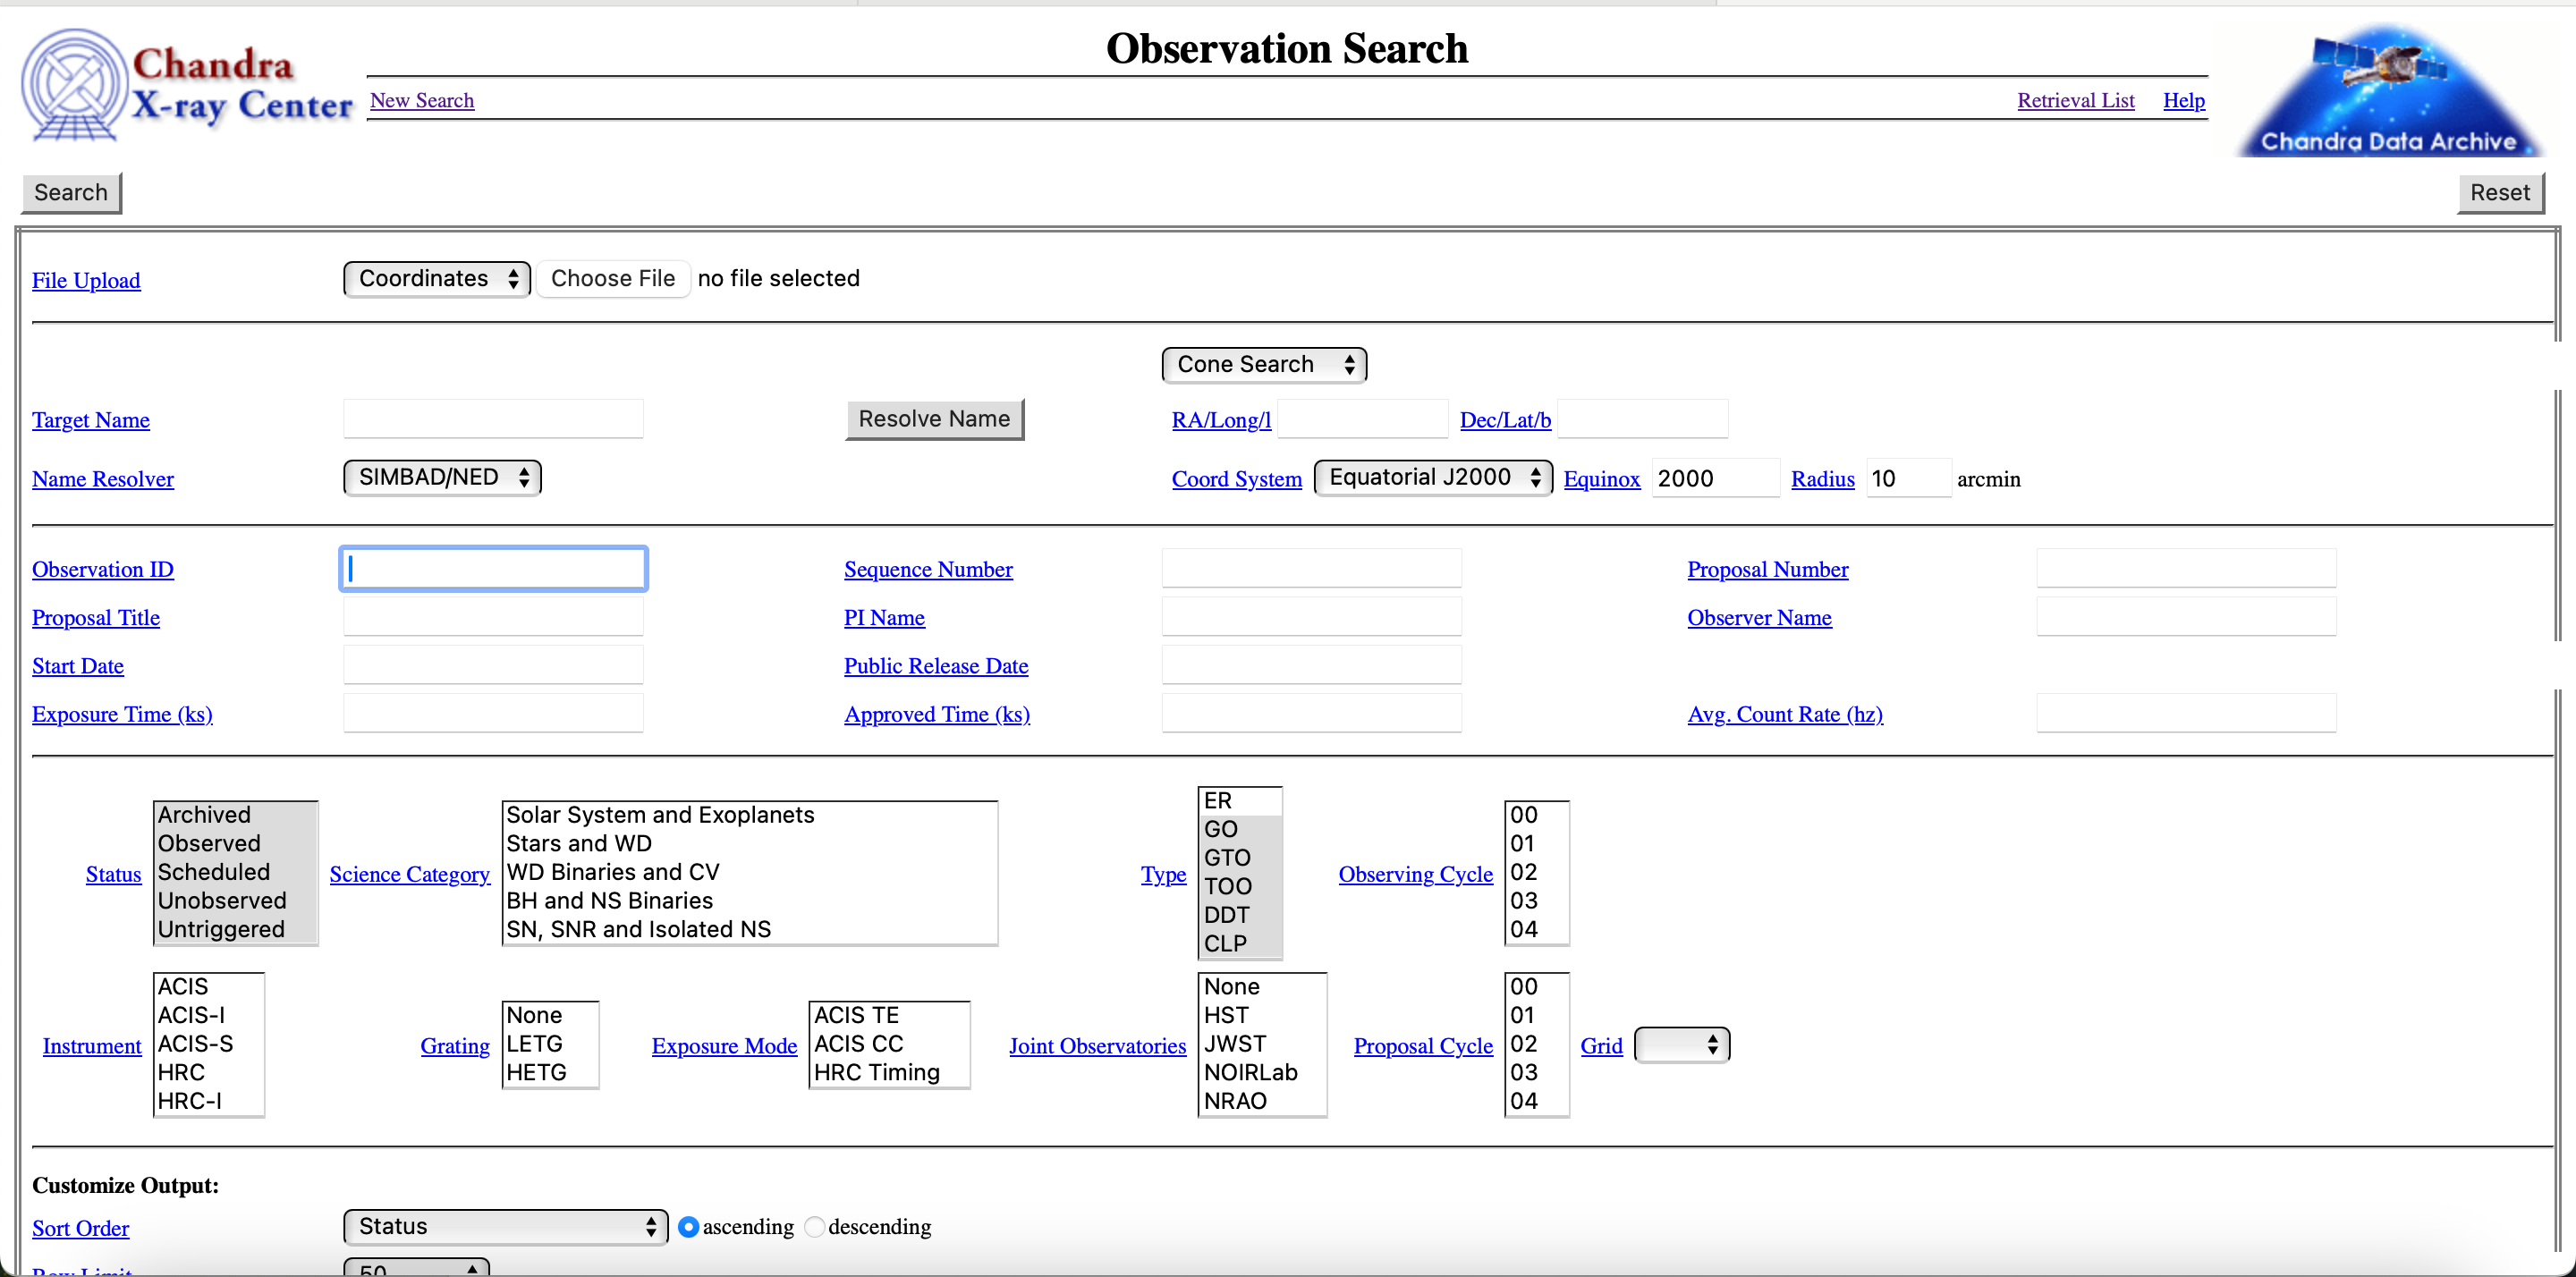
\includegraphics[width=\linewidth]{data_retrival.png}
    \caption{Web based Data Retrival tool}
    \label{fig:Chanda Archive reterival tool}
\end{figure}

\begin{figure}[h!]
    \centering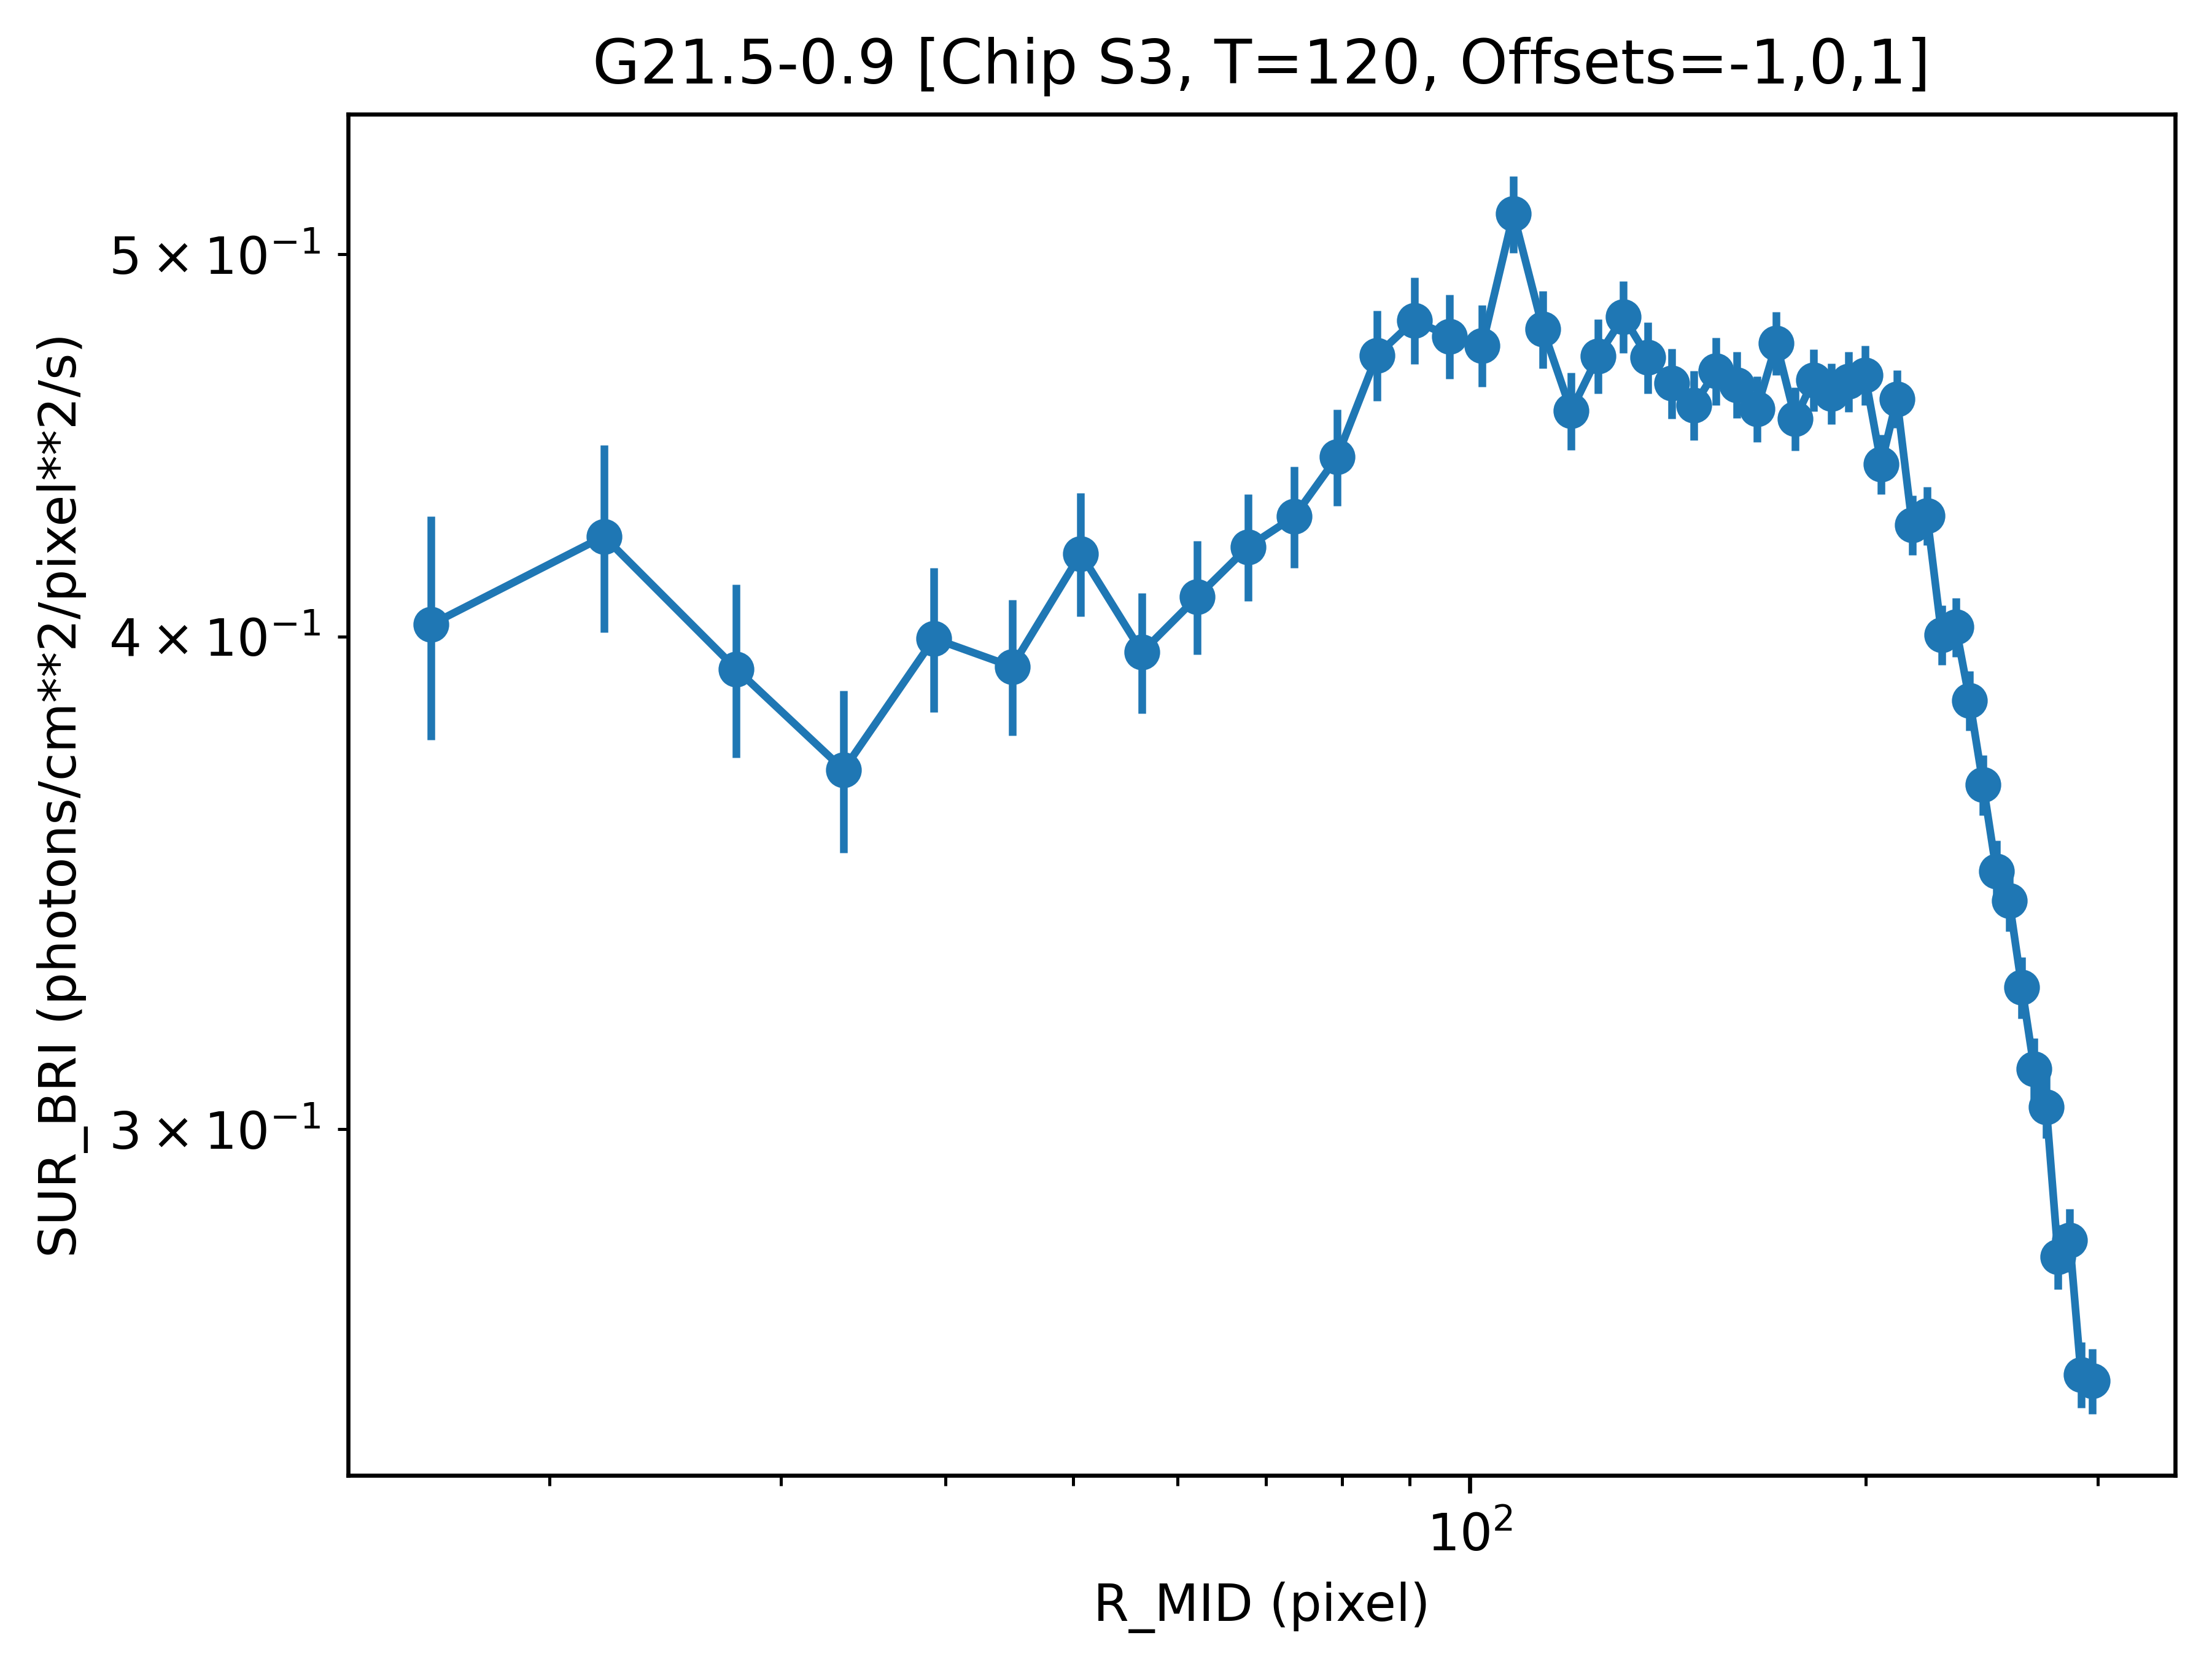
\includegraphics[width=\linewidth]{surface_brightness.png}
    \caption{Surface Brightness curve}
    \label{fig:Radial Profile Fit}
\end{figure}

\begin{figure}[h!]
    \centering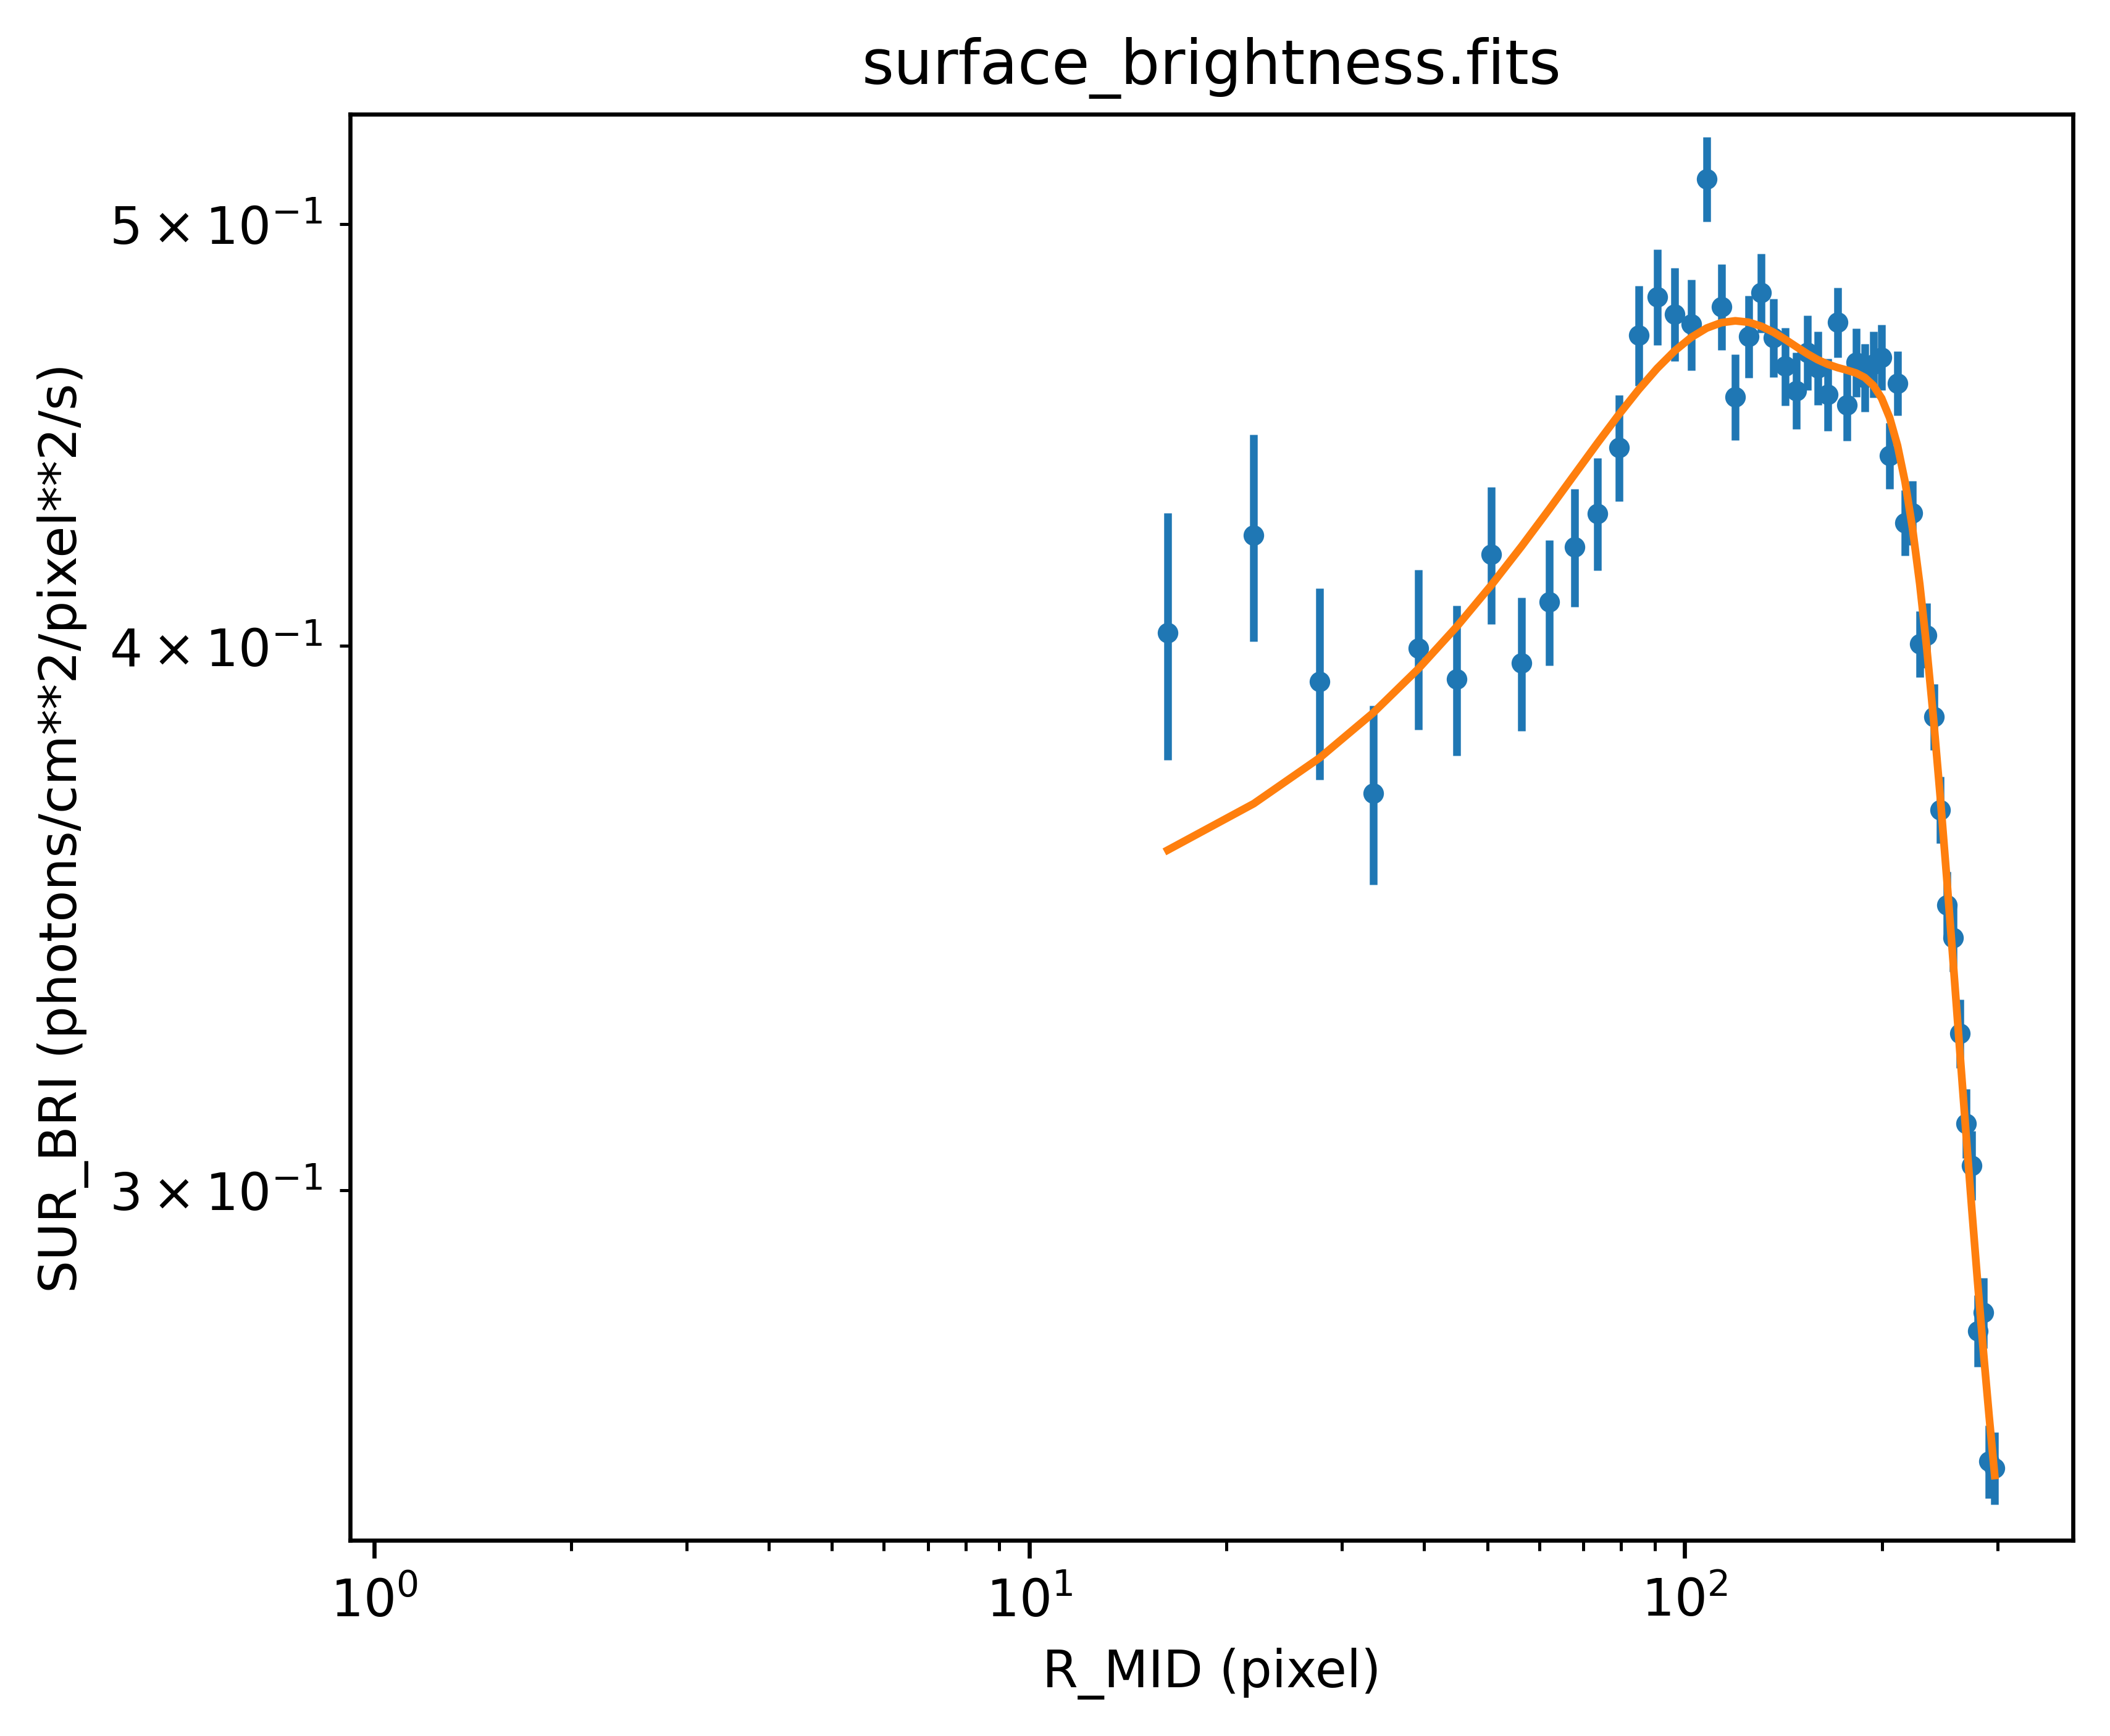
\includegraphics[width=\linewidth]{beta_gauss_fit.png}
    \caption{Using normalized beta + gauss model}
    \label{fig:Beta Gauss Model}
\end{figure}

\begin{figure}[h!]
    \centering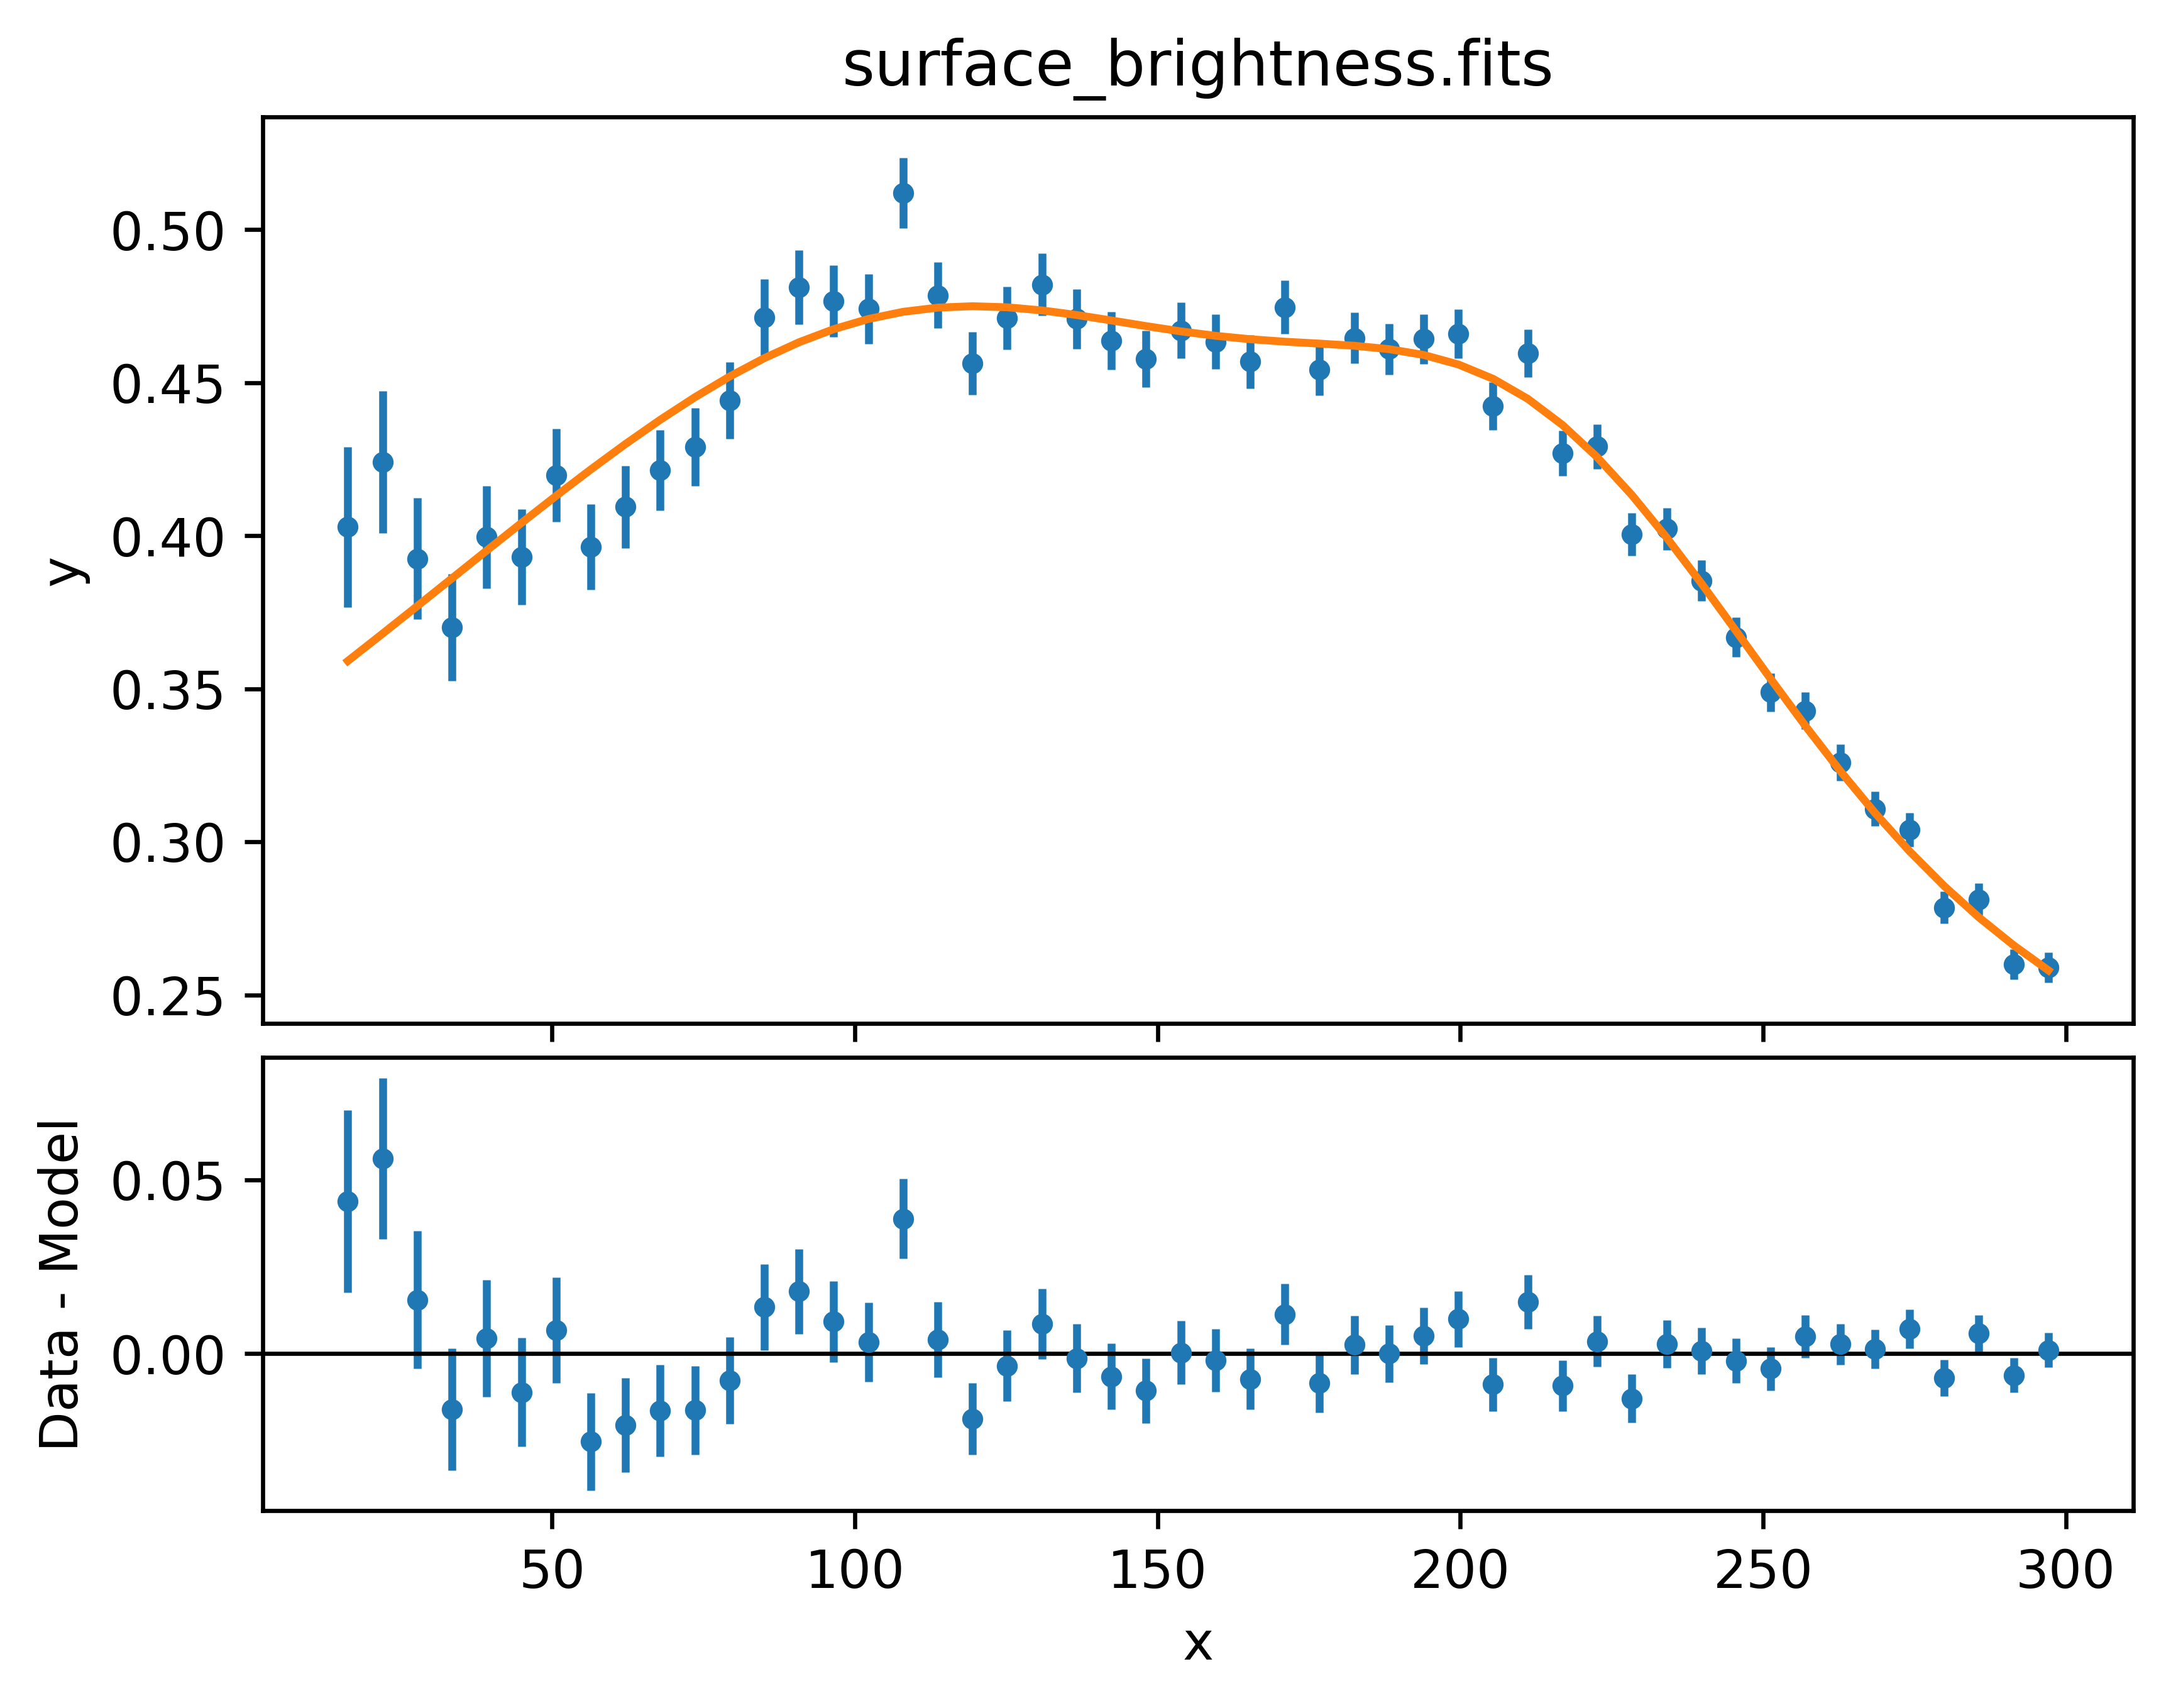
\includegraphics[width=\linewidth]{beta_gauss_resid.png}
    \caption{Error Residual Plot for Beta + gauss model}
    \label{fig:Beta Gauss Resid}
\end{figure}

\appendix
\section{Appendix: Tables}

\begin{table}[h]
    \centering
    \caption{Observation Details for A2163 (Observation ID: 545 and 1653)}
    \begin{tabular}{ll|ll}
        \toprule
        \multicolumn{2}{c|}{\textbf{Observation ID: 545}} & \multicolumn{2}{c}{\textbf{Observation ID: 1653}} \\
        \midrule
        \textbf{Sequence Number} & 800053 & \textbf{Sequence Number} & 800121 \\
        \textbf{Type} & GTO & \textbf{Type} & GTO \\
        \textbf{PI Name} & VANSPEYBROECK & \textbf{PI Name} & Murray \\
        \textbf{Science Category} & Clusters of Galaxies & \textbf{Science Category} & Clusters of Galaxies \\
        \textbf{Target Name} & A2163 & \textbf{Target Name} & Abell 2163 \\
        \textbf{RA (J2000)} & 16 15 45.77 & \textbf{RA (J2000)} & 16 15 45.77 \\
        \textbf{Dec (J2000)} & -06 08 55.00 & \textbf{Dec (J2000)} & -06 08 55.00 \\
        \midrule
        \textbf{Instrument} & ACIS-I & \textbf{Instrument} & ACIS-I \\
        \textbf{Grating} & NONE & \textbf{Grating} & NONE \\
        \textbf{Data Mode} & VFAINT & \textbf{Data Mode} & VFAINT \\
        \textbf{Status} & Archived & \textbf{Status} & Archived \\
        \textbf{Proposal Number} & 01800146 & \textbf{Proposal Number} & 02800085 \\
        \textbf{Proposal Cycle} & 01 & \textbf{Proposal Cycle} & 02 \\
        \textbf{Observer} & Jones & \textbf{Observer} & Vikhlinin \\
        \textbf{Joint Observatories} & None & \textbf{Joint Observatories} & None \\
        \midrule
        \textbf{Start Date} & 2000-07-29 11:09:58 & \textbf{Start Date} & 2001-06-16 11:38:07 \\
        \textbf{Approved Time} & 10.00 ks & \textbf{Approved Time} & 80.00 ks \\
        \textbf{Exposure Time} & 9.45 ks & \textbf{Exposure Time} & 71.15 ks \\
        \textbf{Observing Cycle} & 01 & \textbf{Observing Cycle} & 02 \\
        \textbf{Public Release Date} & 2001-08-07 08:45:00 & \textbf{Public Release Date} & 2002-06-21 10:00:00 \\
        \bottomrule
    \end{tabular}
    \label{tab: Data Product details}
\end{table}

\begin{table}[h]
    \centering
    \caption{Current X-ray Centroid vs. Brightest X-ray Pixel (From dmstat)}
    \begin{tabular}{|c|c|c|}
        \toprule
         \textbf{Measurement} & \textbf{X (Physical} & \textbf{Y (Physical}\\
         \midrule
         X-ray Centroid (dmstat centroid=yes) & 4067.21 & 4267.06 \\
         \midrule
         Brightest X-ray Pixel (dmstat centroid=no) & 3687 & 5076\\
         \bottomrule
    \end{tabular}
    \label{tab:Centroid comparision for A2163}
\end{table}
\end{document}